\section{Data and sample selection}
\label{sec:sample}
The MaNGA (Mapping Nearby Galaxies at Apache Point Observatory; \citet{2015ApJ...798....7B}. [You have duplicated some text from the introduction.]
\subsection{Sample collection}
Include a write-up here on the conditions for identifying a post-starburst galaxy or region. Here is a starter for ten. Check this carefully with Chen et al. (2019) for consistency.
\begin{enumerate}
    \item H$\delta$ absorption line features
    \item strong 4000 \AA\ break 
    \item absence of H$\alpha$ emission lines
    \item at least 6 contiguous spaxels...
    \item 
\end{enumerate}

AN example of the spectrum of a PSB galaxy exhibiting central PSB features is shown in Figure \begin{figure}
    \centering
    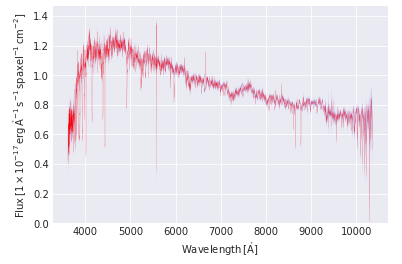
\includegraphics[width=\columnwidth]{images/Spectra/8623-9102.png}
    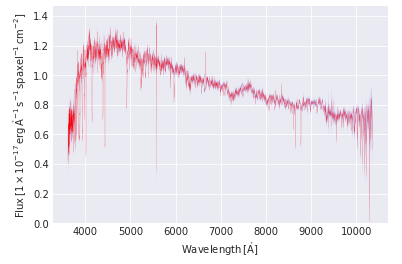
\includegraphics[width=\columnwidth]{images/Spectra/8623-9102.png}
    \caption{Top: typical spectrum of the central spaxel of a CPSB, in this example 8623-9102. Note the strong hydrogen absorption line features in the 3500 to 4500 \AA\ region.
    Bottom: TODO include spectrum of CPSB control galaxy.}
    \label{fig:CPSB-8623-9102-spec}
\end{figure}

\subsection{CPSBs}
The PSB galaxy sample selection process described in Section \ref{sec:sample} on the MaNGA MPL-6 data release yielded a total of 31 galaxies with central post-starburst features, as listed in Table \ref{tab:my-CPSBs}.

\begin{table}
\caption{Central-type PSBs from MaNGA MPL-6}
\label{tab:my-CPSBs}
\begin{tabular}{lccccc}
\hline
PlateIFU & RA & dec & z & log & S\'ersic\\
& & & & $M_*$ & n \\
\hline
7443-12701 & 230.50746 & 43.53234 & 0.020 & 9.693 & 4.43 \\
7964-1902 & 317.42261 & 0.62777 & 0.024 & 9.423 & 6.00 \\
8080-3702 & 49.22887 & -0.04201 & 0.023 & 9.877 & 5.91 \\
8081-3702 & 49.94685 & 0.62382 & 0.025 & 9.145 & 3.42 \\
8082-3704 & 50.88860 & -0.43854 & 0.024 & 9.761 & 2.51 \\
8143-3703 & 120.63984 & 42.39270 & 0.041 & 9.796 & 3.78 \\
8144-1902 & 114.45795 & 28.65289 & 0.016 & 8.799 & 1.48 \\
8313-6101 & 240.65805 & 41.29343 & 0.035 & 10.308 & 6.00 \\
8315-3703 & 236.16573 & 38.42536 & 0.076 & 11.025 & 5.54 \\
8331-6104 & 206.29627 & 42.31951 & 0.028 & 9.792 & 2.22 \\
8555-3701 & 246.76069 & 43.47610 & 0.046 & 10.601 & 3.82 \\
8623-9102 & 311.76380 & 0.43678 & 0.013 & 9.332 & 2.00 \\
8655-1902 & 358.46882 & -0.09873 & 0.022 & 9.241 & 1.82 \\
8713-3701 & 117.06113 & 39.04573 & 0.014 & 8.820 & 0.84 \\
8725-1902 & 127.48937 & 44.94016 & 0.043 & 10.513 & 4.05 \\
8933-3704 & 195.33050 & 27.86046 & 0.027 & 9.117 & 3.19 \\
8934-9101 & 196.26374 & 27.53704 & 0.022 & 9.086 & 6.00 \\
8935-12701 & 194.52342 & 29.01735 & 0.026 & 9.259 & 1.82 \\
8938-6102 & 120.06709 & 29.47144 & 0.045 & 9.823 & 3.34 \\
8941-3701 & 120.05960 & 26.69801 & 0.028 & 10.031 & 4.79 \\
8944-1902 & 148.42110 & 35.70188 & 0.040 & 9.590 & 5.93 \\
8950-3704 & 194.33162 & 27.61386 & 0.026 & 9.086 & 1.74 \\
8979-1902 & 242.58533 & 41.85490 & 0.040 & 10.634 & 6.00 \\
8996-3704 & 173.41287 & 52.67459 & 0.049 & 10.094 & 5.08 \\
8997-3703 & 170.72345 & 51.34178 & 0.034 & 9.600 & 1.25 \\
9047-3701 & 246.48074 & 25.41161 & 0.039 & 9.773 & 4.21 \\
9085-1902 & 260.61132 & 28.30970 & 0.069 & 10.662 & 6.00 \\
9493-12705 & 129.99929 & 23.41340 & 0.012 & 8.916 & 0.77 \\
9494-3701 & 126.75586 & 21.70675 & 0.015 & 9.949 & 1.96 \\
9494-3703 & 127.31796 & 23.80902 & 0.018 & 9.168 & 5.43 \\
9876-12701 & 194.63449 & 28.37796 & 0.020 & 8.851 & 5.05 \\
\hline
\end{tabular}
\end{table}

An example of the MaNGA stellar velocity and gas velocity maps for a CPSB is illustratred in Figure \begin{figure}
    \centering
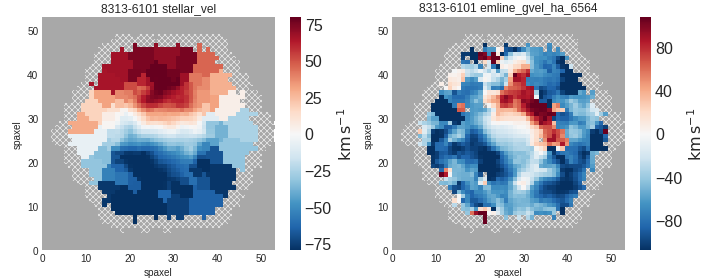
\includegraphics[width=\columnwidth]{images/VelocityMaps/CPSB-8313-6101-VMAPS.png}
    \caption{MaNGA velocity maps for CPSB 8313-6101: stellar velocity (left) and H$\alpha$ gas velocity (right).}
    \label{fig:CPSB-8313-6101-VMAPS}
\end{figure}

\subsection{RPSBs}
Similarly the PSB galaxy sample selection process described in Section \ref{sec:sample} on the MaNGA MPL-6 data release yielded a total of 37 galaxies with ring-like post-starburst features, as listed in Table \ref{tab:my-RPSBs}.

\begin{table}
\caption{Ring-type PSBs from MaNGA MPL-6}
\label{tab:my-RPSBs}
\begin{tabular}{lccccc}
\hline
PlateIFU & RA & dec & z & log & S\'ersic \\
& & & & $M_*$ & n \\
\hline
8080-3704 & 49.45745 & -0.55466 & 0.021 & 9.790 & 1.58 \\
8083-12703 & 49.92934 & 0.56548 & 0.024 & 9.960 & 3.80 \\
8085-6104 & 51.70891 & 0.19859 & 0.020 & 9.538 & 6.00 \\
8146-1901 & 117.05387 & 28.22509 & 0.027 & 9.907 & 1.71 \\
8250-6101 & 138.75315 & 42.02439 & 0.028 & 10.054 & 2.40 \\
8250-6104 & 140.41142 & 43.72615 & 0.040 & 10.383 & 1.47 \\
8255-3703 & 166.18780 & 45.15643 & 0.022 & 9.271 & 2.44 \\
8261-6103 & 181.54597 & 45.14921 & 0.067 & 10.583 & 4.76 \\
8262-3701 & 183.57898 & 43.53528 & 0.024 & 9.452 & 2.21 \\
8274-12701 & 164.58519 & 40.78823 & 0.026 & 9.314 & 0.85 \\
8322-1901 & 198.78425 & 30.40377 & 0.023 & 10.011 & 2.44 \\
8323-6103 & 196.10272 & 36.47995 & 0.023 & 9.858 & 1.35 \\
8439-6104 & 143.51035 & 50.02749 & 0.038 & 10.453 & 3.36 \\
8440-1901 & 136.11419 & 41.48621 & 0.024 & 9.067 & 2.20 \\
8440-6104 & 135.75897 & 40.43399 & 0.029 & 10.415 & 5.31 \\
8453-3704 & 154.48083 & 46.60329 & 0.030 & 9.782 & 1.78 \\
8458-6102 & 147.66431 & 44.33116 & 0.015 & 9.399 & 1.58 \\
8486-1901 & 238.44858 & 47.40496 & 0.019 & 9.226 & 1.39 \\
8547-9102 & 218.97634 & 53.39164 & 0.043 & 9.977 & 1.37 \\
8554-3701 & 183.00790 & 35.40440 & 0.024 & 9.657 & 2.67 \\
8604-3702 & 247.14945 & 39.71974 & 0.037 & 9.462 & 0.76 \\
8655-3701 & 356.75183 & -0.44739 & 0.071 & 10.729 & 3.34 \\
8932-12704 & 196.47287 & 28.11243 & 0.025 & 9.805 & 1.99 \\
8943-1901 & 154.97835 & 36.32574 & 0.026 & 9.854 & 3.10 \\
8950-12705 & 194.73314 & 27.83344 & 0.025 & 10.265 & 0.96 \\
8950-6101 & 194.76938 & 26.95819 & 0.027 & 9.137 & 2.66 \\
8982-6104 & 203.05706 & 26.94998 & 0.035 & 10.222 & 1.52 \\
8987-9102 & 137.98351 & 27.89927 & 0.047 & 10.080 & 1.45 \\
8997-3704 & 171.77902 & 51.13164 & 0.015 & 9.027 & 2.25 \\
9181-12705 & 120.55787 & 37.15008 & 0.084 & 10.664 & 1.68 \\
9184-3703 & 119.36531 & 33.25794 & 0.017 & 8.949 & 1.56 \\
9194-3702 & 47.02945 & 0.45621 & 0.074 & 10.623 & 4.82 \\
9487-9102 & 123.82033 & 46.07525 & 0.041 & 10.503 & 5.88 \\
9505-6102 & 139.17787 & 28.05423 & 0.028 & 9.708 & 1.15 \\
9868-3702 & 218.94756 & 47.00747 & 0.027 & 9.457 & 1.70 \\
9872-3701 & 233.23196 & 42.43826 & 0.020 & 9.745 & 2.28 \\
9891-6102 & 228.41485 & 28.24446 & 0.046 & 9.766 & 1.42 \\
\hline
\end{tabular}
\end{table}

\subsection{Control galaxies}
Control galaxies as 'normal' galaxies not exhibiting PSB features. Also check this with Chen et al. (2019) for consistency.

\subsection{Quality screening}
We will need a short write-up from Chris on the quality flag screening of the MPL-8 data release.



\subsection{PA plots: misaligned CPSBs}
[Include a few examples of the PDF output from kinemetry: Chris' plots.]

\begin{figure}
    \centering
    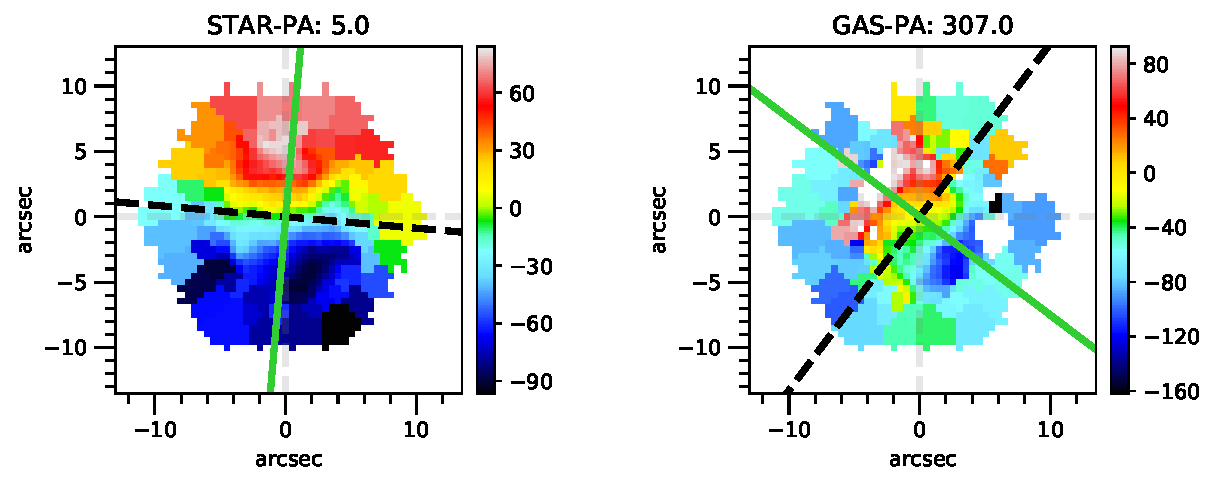
\includegraphics[width=\columnwidth]{images/PAplots/PAplotsCPSB/8313-6101-PA.pdf}
    \caption{Kinemetry-derived stellar and gas velocity position angles for CPSB-8313-6101.}
    \label{fig:CPSB-8313-6101-PA}
\end{figure}

\begin{table}
\caption{CPSBs with PA offset \textgreater 30 deg.}
\label{tab:offsetCPSBs}
\begin{tabular}{lccc}
\hline
PlateIFU  & Stellar PA & H$\alpha$ PA & $\Delta$PA \\
  & (deg.) & (deg.) & (deg.) \\
\hline
8313-6101 & 5 & 307 & 58 \\
8655-1902 & 335 & 127 & 152 \\
8725-1902 & 22 & 175 & 153 \\
8938-6102 & 214 & 47.5 & 166.5 \\
9494-3701 & 140.5 & 243 & 102.5 \\
\hline
\end{tabular}
\end{table}

\subsection{PA plots: misaligned RPSBs}

\begin{table}
\caption{RPSBs with PA offset \textgreater 30 deg.}
\label{tab:offsetRPSBs}
\begin{tabular}{lccc}
\hline
PlateIFU   & Stellar PA & H$\alpha$ PA & $\Delta$PA \\
  & (deg.) & (deg.) & (deg.) \\
\hline
8080-3704 & 24 & 154 & 130 \\
8262-3701 & 153.5 & 118.5 & 35 \\
8323-6103 & 109.5 & 313.5 & 156 \\
8439-6104 & 5.5 & 107 & 101.5 \\
8453-3704 & 44 & 91 & 47 \\
8486-1901 & 295.5 & 85 & 149.5 \\
8554-3701 & 250 & 68 & 178 \\
8932-12704 & 166.5 & 134.5 & 32 \\
9872-3701 & 208.5 & 81 & 127.5 \\
\hline
\end{tabular}
\end{table}

